\documentclass[../main.tex]{subfiles}

\begin{document}
	\section{Esercizio}
	Calcolare tutte le possibili funzioni di trasferimento del sistema:
	\begin{figure}[h!]
		\centering
		\begin{subfigure}{0.8\textwidth}
			\includegraphics[width=\textwidth]{interconnections/algebra_blocchi_es1_1}
		\end{subfigure}%
	\end{figure}
	\begin{itemize}
		\item $ T_{y_1 u_1}(s) $: poniamo $ u_2 = 0 $.\\
		\parbox[t]{\dimexpr\textwidth-\leftmargin}{%
			\vspace{-2.5mm}
			\begin{wrapfigure}{r}{0.5\textwidth}
				\centering
				\vspace{-\baselineskip}
				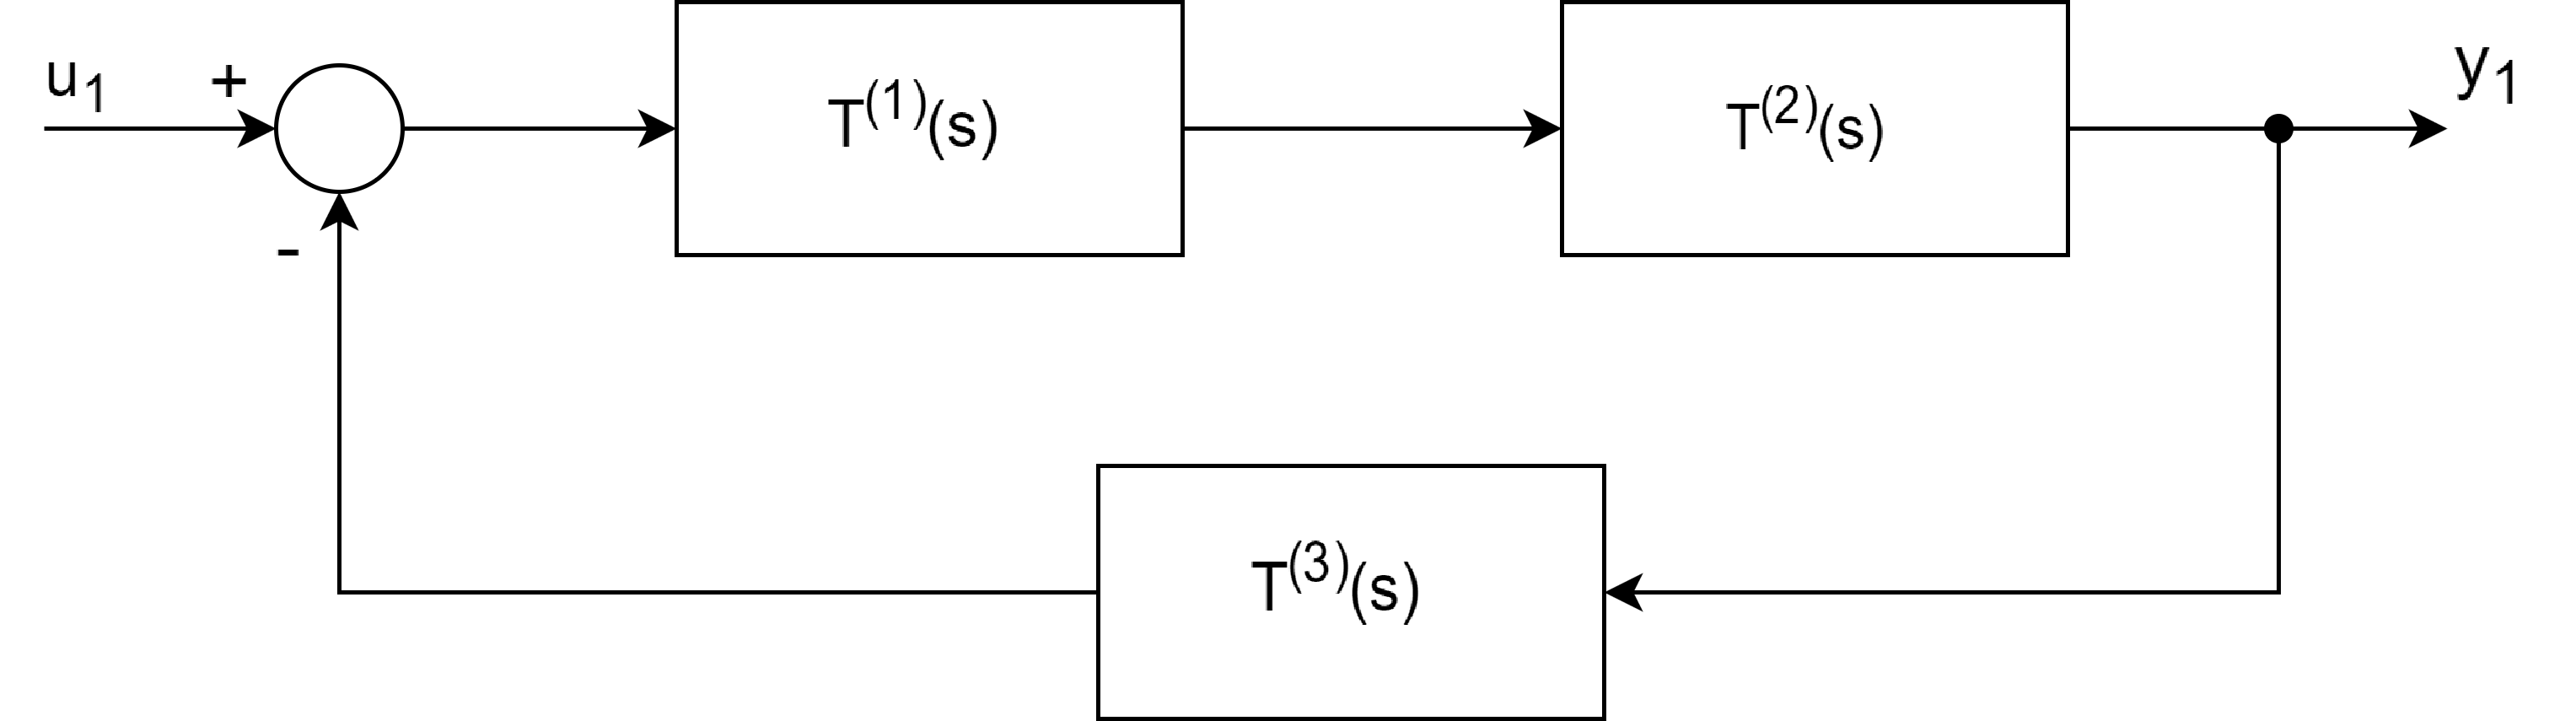
\includegraphics[width=\linewidth]{interconnections/algebra_blocchi_es1_2}
			\end{wrapfigure}
			Serie tra $ T^{(1)} $ e $ T^{(2)} $:
			\[ T_{serie} = T^{(1)} T^{(2)} = \frac{s+1}{s-1} \frac{1}{s+1} = \frac{1}{s-1} \]
			Retroazione tra $ T_{serie} $ e $ T^{(3)} $:
			\[ T_{y_1 u_1}(s) = \frac{T_{serie}}{1+T_{serie} T^{(3)}} = \frac{\frac{1}{s-1}}{1+\frac{1}{(s+1)(s-1)}} = \frac{\frac{1}{s-1}}{\frac{1}{(s^2-1+1)(s-1)}} = \frac{s+1}{s^2} \]
			Questa funzione di trasferimento \'e instabile BIBO perch\'e c'\'e un polo a $ \Re = 0 $.
		}
		%
		\item $ T_{y_1 u_2}(s) $: poniamo $ u_1 = 0 $.\\
		\parbox[t]{\dimexpr\textwidth-\leftmargin}{%
			\vspace{-2.5mm}
			\begin{wrapfigure}[10]{r}{0.5\textwidth}
				\centering
				\vspace{-\baselineskip}
				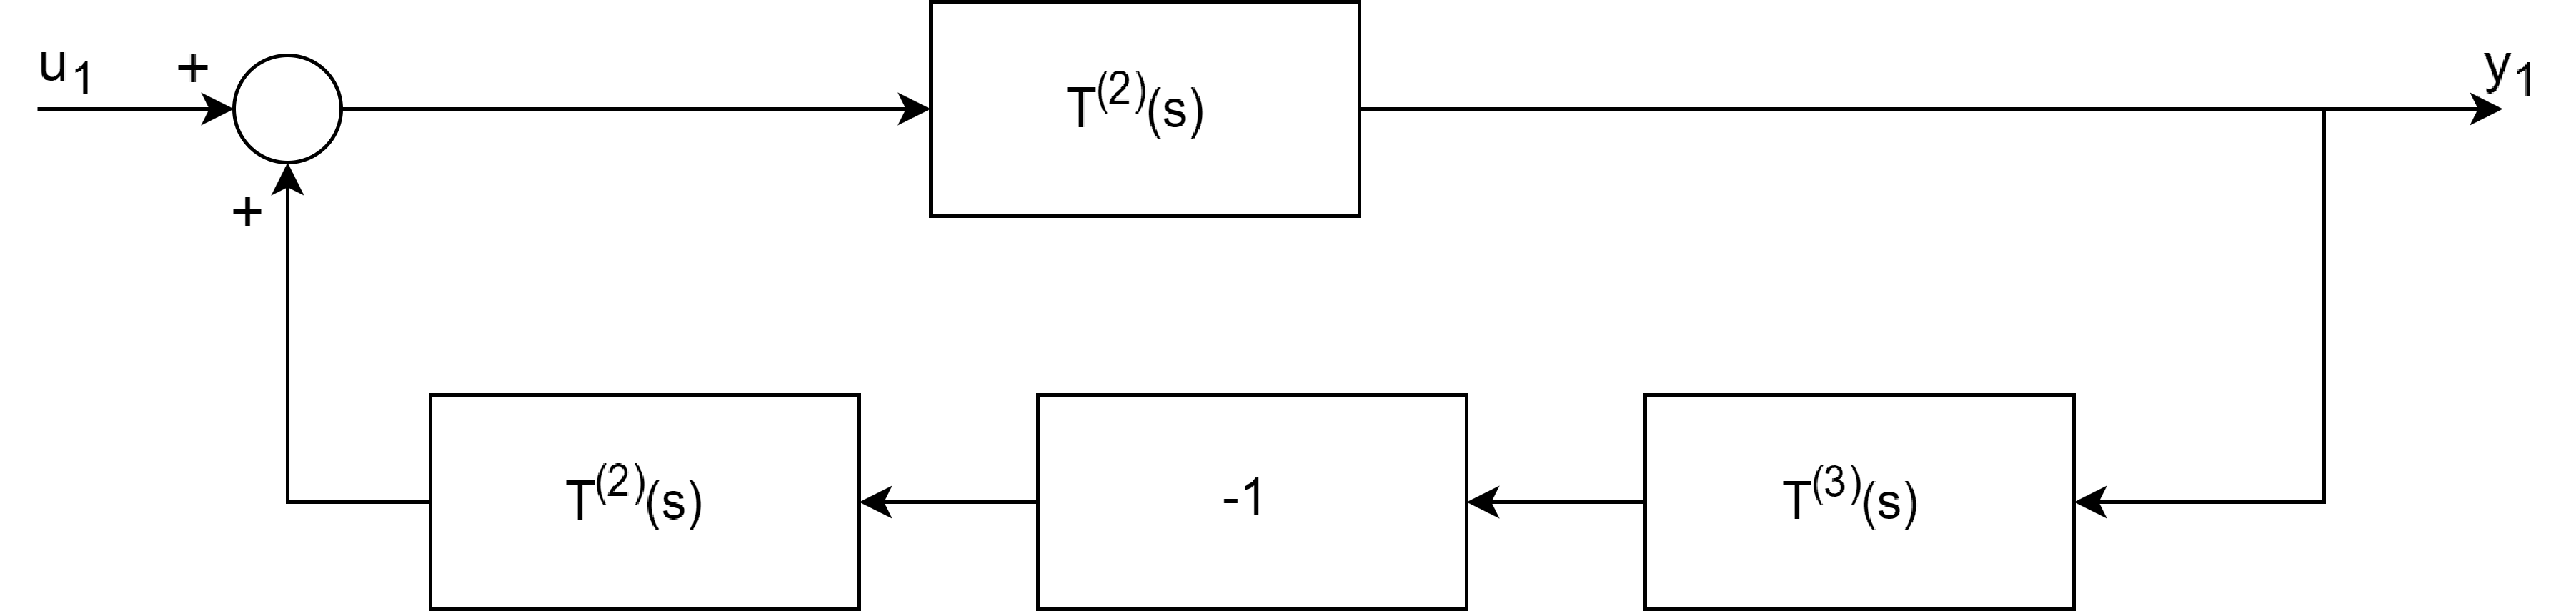
\includegraphics[width=\linewidth]{interconnections/algebra_blocchi_es1_3}
			\end{wrapfigure}
			Calcoliamo la serie nella catena inversa di retroazione:
			\[ T_{serie}(s) = \frac{-1}{(s+1)^2} \]
			Retroazione:
			\[ T_{y_1 u_2}(s) = \frac{\frac{s+1}{s-1}}{1-\frac{s+1}{s-1}\frac{-1}{(s+1)^2}} = \frac{\frac{s+1}{s-1}}{1+\frac{1}{(s+1)(s-1)}} = \frac{\frac{s+1}{s-1}}{\frac{s^2}{(s+1)(s-1)}} = \frac{(s+1)^2}{s^2} \]
			Questa funzione di trasferimento \'e instabile BIBO perch\'e c'\'e un polo a $ \Re = 0 $.
			Abbiamo ottenuto una funzione di trasferimento semplicemente propria perch\'e tra $ u_2 $ e $ y_1 $ in catena diretta c'\'e una dipendenza istantanea (dato dalla costante):
			\[ T^{(2)}(s) = \frac{s+1}{s-1} = 1 + \frac{2}{s-1} \]
		}
		%
		\item $ T_{y_2 u_1}(s) $:
		\[ T_{y_2 u_1}(s) = \frac{\frac{s+1}{s-1}\frac{1}{s+1}}{1+\frac{s^2}{(s+1)(s-1)}} = \frac{1}{s^2} \]
		%
		\item $ T_{y_2 u_2}(s) $:
		\[ T_{y_2 u_2}(s) = \frac{\frac{1}{s-1}}{\frac{s^2}{(s+1)(s-1)}} = \frac{s+1}{s^2}\]
	\end{itemize}
	%
	\section{Esercizio}
	Calcolare la funzione di trasferimento del sistema:\\
	\begin{figure}[h!]
		\centering
		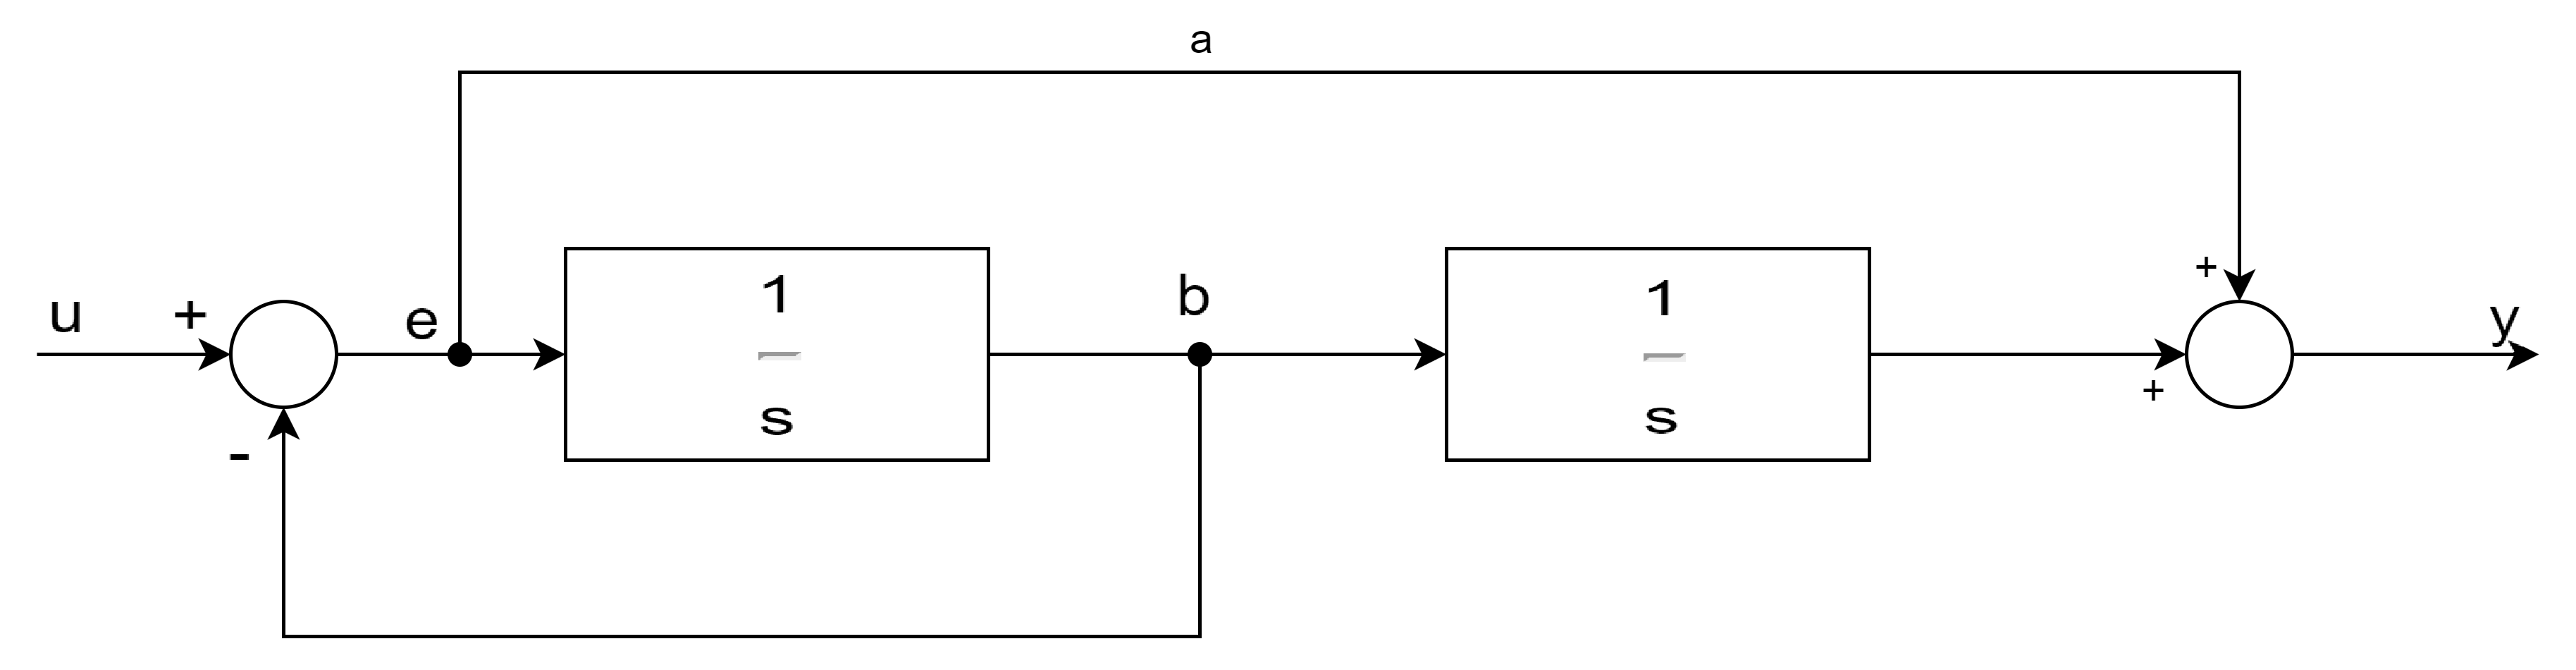
\includegraphics[width=\textwidth]{interconnections/algebra_blocchi_es2_1}
	\end{figure}

	Spostiamo il nodo $ e $ e otteniamo un nuovo sistema composto da una retroazione e da un parallelo.
	L'algebra dei blocchi permette di fare queste equivalenze solo per il calcolo della funzione di trasferimento complessiva e non per altri calcoli, perch\'e stiamo introducendo nuovi blocchi, tra cui alcuni irrealizzabili (vedi il blocco di funzione di trasferimento $ s $).
	\begin{figure}[h!]
		\centering
		\begin{subfigure}{0.5\textwidth}
			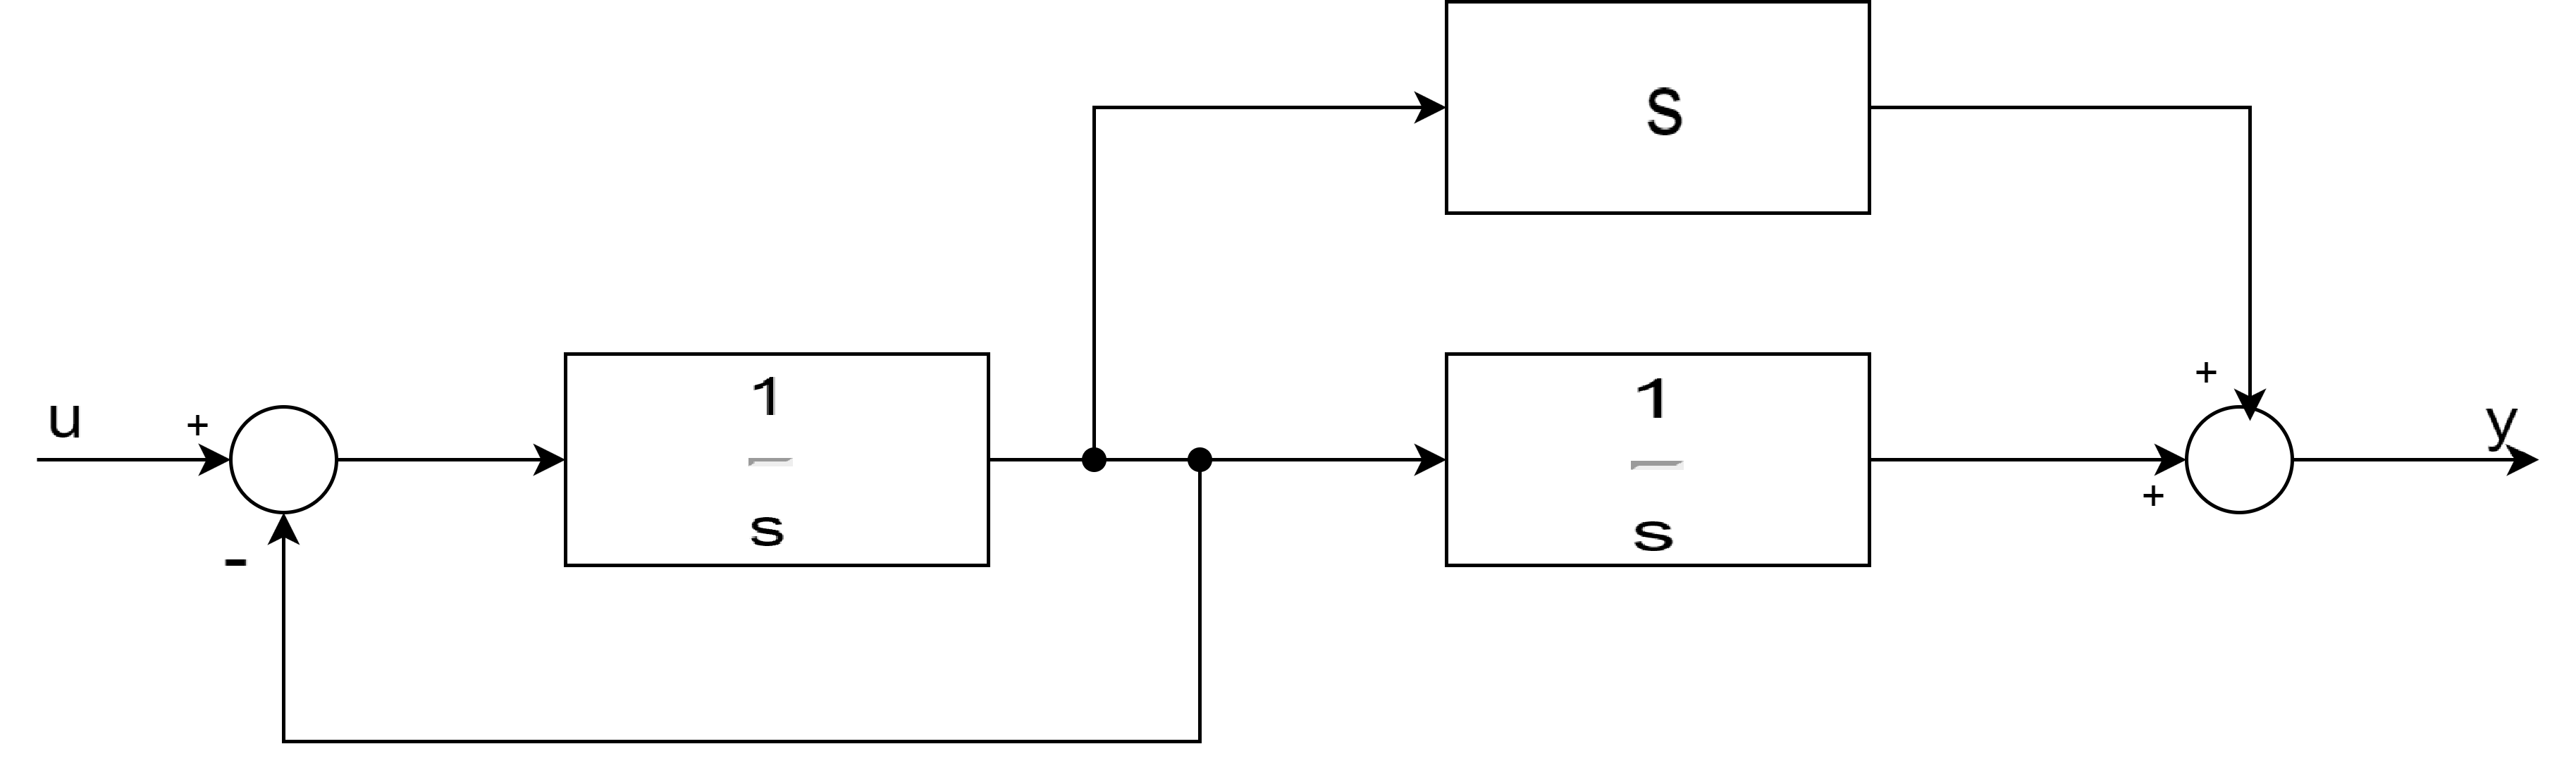
\includegraphics[width=\textwidth]{interconnections/algebra_blocchi_es2_2}
		\end{subfigure}%
		\begin{subfigure}{0.5\textwidth}
			\includegraphics[width=\textwidth]{interconnections/algebra_blocchi_es2_3}
		\end{subfigure}%
	\end{figure}
	\[ T_{yu}(s) = \frac{\frac{1}{s}}{1+\frac{1}{s}} \left( s+\frac{1}{s} \right) = \frac{s^2+1}{s(s+1)} \]
\end{document}